\documentclass[10pt]{article}
\usepackage[letterpaper,margin=0.9in]{geometry}
\usepackage[T1]{fontenc}
\usepackage{newtxtext,newtxmath}
\usepackage{graphicx,booktabs,microtype,xcolor,enumitem,tabularx}
\usepackage[skins,breakable]{tcolorbox}
\usepackage[hidelinks]{hyperref}
\usepackage{titlesec,needspace}
\usepackage[font=small,labelfont=bf,labelsep=period]{caption}

\definecolor{ink}{HTML}{1F2328}
\definecolor{rule}{HTML}{D0D7DE}
\definecolor{pinkish}{HTML}{D6336C}
\definecolor{panel}{HTML}{F6F8FA}

\titleformat{\section}{\needspace{4\baselineskip}\large\bfseries\color{ink}}{}{0pt}{}
\titleformat{\subsection}{\normalsize\bfseries\color{ink}}{}{0pt}{}
\titlespacing*{\section}{0pt}{9pt}{3pt}
\titlespacing*{\subsection}{0pt}{6pt}{2pt}
\setlist{nosep,leftmargin=1.2em}
\setlength{\parskip}{3pt}
\setlength{\parindent}{0pt}
\setlength{\textfloatsep}{8pt}
\setlength{\floatsep}{6pt}

\newtcolorbox{methods}[1][]{enhanced,breakable,colback=panel,colframe=panel,boxrule=0pt,
  left=6pt,right=6pt,top=4pt,bottom=4pt,arc=0pt,fontupper=\small,
  borderline west={1.5pt}{0pt}{pinkish},title={\textbf{#1.}\enspace},attach title to upper,coltitle=ink}

\newcommand{\astraHitCI}{24--61\%}
\newcommand{\astraHits}{10}
\newcommand{\astraLeakCI}{62--98\%}
\newcommand{\astraLeaks}{10}
\newcommand{\astraMaxOther}{2}
\newcommand{\astraOther}{0}
\newcommand{\contrHitCI}{64--93\%}
\newcommand{\contrLeakCI}{2--38\%}
\newcommand{\contrastiveConstraints}{224}
\newcommand{\contrastiveHits}{20}
\newcommand{\contrastiveLeaks}{1}
\newcommand{\contrastiveLmControls}{6}
\newcommand{\contrastiveLmHits}{5}
\newcommand{\contrastiveLone}{763}
\newcommand{\contrastiveOther}{0}
\newcommand{\convHitCI}{69--96\%}
\newcommand{\convLeakCI}{28--79\%}
\newcommand{\convVsAstraB}{11}
\newcommand{\convVsAstraC}{0}
\newcommand{\convVsAstraP}{0.0010}
\newcommand{\conventionalHits}{21}
\newcommand{\conventionalLeaks}{6}
\newcommand{\conventionalMaxOther}{1}
\newcommand{\conventionalOther}{0}
\newcommand{\extControls}{24}
\newcommand{\extNaming}{11}
\newcommand{\extOther}{13}
\newcommand{\extTargets}{24}
\newcommand{\floorDdr}{6.19}
\newcommand{\floorMac}{1.92}
\newcommand{\latArray}{132.1}
\newcommand{\latBaseline}{797.5}
\newcommand{\latBestMax}{16.16}
\newcommand{\latBestMin}{14.30}
\newcommand{\latLadderSpeedup}{16}
\newcommand{\latQueue}{49.9}
\newcommand{\latScalarMax}{43.41}
\newcommand{\latScalarMin}{40.39}
\newcommand{\latVerifyMax}{24.70}
\newcommand{\latVerifyMin}{19.65}
\newcommand{\lmAstraCI}{19--81\%}
\newcommand{\lmBoardMatchesSoftware}{yes}
\newcommand{\lmBoardScores}{925{,}696}
\newcommand{\lmConvCI}{44--97\%}
\newcommand{\weightGB}{2.45}


\begin{document}

{\small\color{pinkish}\textbf{November 22, 2026} \quad Technical report \quad Hardware $\cdot$ Model editing}

\vspace{4pt}
{\LARGE\bfseries\color{ink} Editing and serving a language model on a PYNQ-Z2 FPGA:\\[2pt] bit-exact parity, reversible weight edits and a 16$\times$ faster diagnosis}

\vspace{6pt}
{\normalsize Stefan Ilas \quad Mohsen Sarrafan Chaharsoughi}\\
{\small pinkProcess \quad \href{https://github.com/StefanIlas1/pinkProcess}{github.com/StefanIlas1/pinkProcess}}

\vspace{6pt}
{\color{rule}\hrule}
\vspace{6pt}

pinkProcess is a Mac app paired with a PYNQ-Z2 board (a Zynq-7020 FPGA with two ARM cores). It answers questions about live service telemetry with a quantized language model that runs on the board. An operator can replace one row of that model's weights while it serves, and restore the original byte for byte. This report covers what we built and what we measured. We describe the inputs (hardware, models, workloads), the process that keeps every number reproducible, and the outputs: numerical parity, weight edits and latency. We also ran three new software experiments for this report. They test whether the board's one-row edits generalize to unseen prompts and how to make them more specific.

\textbf{Our biggest takeaways:}
\begin{itemize}
\item \textbf{The FPGA path is bit-exact.} Every physical comparison matched the integer reference. That covers \lmBoardScores{} classifier scores in the held-out edit study and 842{,}752 scores for the full projection array.
\item \textbf{A 64-byte edit is a real, reversible behavior change, but it edits a \emph{slot}, not a concept.} The conventional row selects the new name on \conventionalHits{} of \extTargets{} unseen target prompts. It also renames \conventionalLeaks{} of \extNaming{} unrelated naming prompts, such as dogs, mothers and trucks. Adding a few contrastive constraints cut that leak to \contrastiveLeaks{} of \extNaming{} while keeping \contrastiveHits{}/\extTargets{} hits. This test was pre-registered and passed.
\item \textbf{Latency fell \latLadderSpeedup$\times$ on one fixed incident, from \latBaseline{} s to \latQueue{} s, and the current backend answers in \latBestMin--\latBestMax{} s.} That is still above our 10-second goal. A memory-traffic bound shows that a full answer at 50\,MHz cannot fall below \floorDdr{} s without changing the memory path.
\end{itemize}

The report follows OpenAI's inputs, process and outputs layout~\cite{openai2026}. Every number is generated from committed evidence by \texttt{paper/analysis.py}.

\section{Inputs}

\subsection{Hardware}
The board is a TUL PYNQ-Z2 (XC7Z020, 53{,}200 LUTs, 140 block RAMs, 220 DSPs) on the stock PYNQ v3.1.1 image. Bitstreams were built with Vivado 2025.2 on an EC2 host. The first overlay missed timing at 100\,MHz by 5.99\,ns and was rebuilt at 50\,MHz. It met timing with 2.07\,ns of setup slack using 1{,}279 LUTs, 8 block RAMs and no DSPs. It holds an AXI INT8 classifier for the output layer. The final overlay adds a DDR-fed $8{\times}8$ signed INT8 array with INT32 accumulation, a command queue and an FP32 vocabulary reducer. It met timing at 50\,MHz with $+2.33$\,ns setup slack using 15{,}959 LUTs, 21 block RAMs and 4 DSPs.

\subsection{Models and workload}
\begin{itemize}
\item \textbf{stories260K}~\cite{karpathy2023llama2c,eldan2023tinystories}: a 5-layer, 260K-parameter TinyStories model with a 512-token vocabulary. It is exported as a 425{,}708-byte integer checkpoint with INT8 weights, Q16 activations and lookup tables for RoPE and the exponent. We use it for the weight-edit studies.
\item \textbf{FLAN-T5-small}~\cite{chung2022flan}, quantized W8A8 and fine-tuned on generated connection-pool incidents. This is the diagnostic model. \emph{Queue history v2} is a separate 360-step checkpoint trained with a short measured-history cue built from the first, peak and latest queue depth.
\item \textbf{Workload:} synthetic SQLite connection-pool telemetry streamed to the board while it answers. The kit also scores each window with a 3-feature fixed-point logistic forecaster. No production traffic was used.
\end{itemize}

\subsection{Weight authors}
Two authors write the edits. The \emph{conventional fit} is an iterative projection that satisfies 60 integer score constraints from an authoring packet. \emph{Astra} is a GPT-6 task given the same packet once and asked to return 64 signed integers directly. Both candidates were hashed and frozen before any held-out prompt was run.

\section{Process}

\subsection{Verification discipline}
Every run pins SHA-256 hashes for the model, tokenizer, bitstream and patch. Each FPGA result is compared integer by integer against an independent C or Python reference. Protocols and candidates are committed before evaluation. Results report numerators and denominators and keep regressions. Table~\ref{tab:parity} lists the parity checks.

\begin{table}[!htb]
\centering\small
\caption{Physical PYNQ-Z2 parity checks. A check passes only if every signed integer score matches the reference.}
\label{tab:parity}
\begin{tabular}{@{}lrl@{}}
\toprule
Check & Scores matched & Scope \\
\midrule
Classifier replay & 17{,}920 & 32 traced activations, row replace and restore \\
Live selective edit & 294{,}912 & 6 prompts $\times$ 3 phases (original, edited, restored) \\
Patch operator & 49{,}152 & Wrong-model and truncated bundles rejected, readback intact \\
LM001 held-out study & \lmBoardScores & 48 runs, every token identical to software \\
Projection array & 842{,}752 & Attention, feed-forward and vocabulary head, 2 shape checks \\
Command queue + reducer & 1{,}160 & Exact winner, earliest index on cross-segment ties \\
\bottomrule
\end{tabular}
\end{table}

\subsection{The edit operation}
An edit is a versioned JSON bundle with the target row, the hashes of the base model, the quantized classifier and the original row, and the replacement bytes. For stories260K this is 64 bytes, a 701-byte bundle. The board checks every hash before writing. It applies the row between requests (0.72\,ms) and verifies it by readback. Rollback rewrites the original row and checks the full classifier hash. Quitting the operator with an edit active also restores the base. On FLAN, the same mechanism writes a 512-byte vocabulary row. Named versions persist across service restarts.

\begin{methods}[Methods: edit experiments]
\emph{LM001} has four conditions: original, a prompt-only instruction, the conventional row and Astra's row. It uses 6 target prompts (``\ldots little girl named'') and 6 controls, with greedy decoding for 20 tokens. A target counts as a \emph{hit} when the first sampled token is \textit{Tim} (token 326). A control counts as \emph{unchanged} when all of its sampled tokens are identical. For this report we froze a new set of 24 target and 24 control prompts in git (commit \texttt{d9b261d}) before running anything. Of the controls, 11 are \emph{naming} prompts (``a big dog named'') and 13 are not. We then swept edit strength $\alpha\in[0,2]$ with row $r_\alpha = \mathrm{clip}(\mathrm{round}(r_0+\alpha(r_1-r_0)))$. The \emph{contrastive fit} reuses the conventional solver and adds 3 authoring-only ``girl named'' positives and 8 ``animal or adult named'' negatives, for 224 constraints. None of these prompts overlaps the held-out sets. Its success criterion ($\ge$18/24 hits, $\le$2/11 naming changes, 0/13 other changes) was committed before the run (\texttt{0891cf9}). Intervals are Wilson 95\%~\cite{wilson1927}. Paired comparisons use exact McNemar tests.
\end{methods}

\section{Outputs}

\subsection{One-row edits change behavior and roll back exactly}
On the board, the selective row changed the first sampled name from \textit{Lily} to \textit{Tim} and the 18 tokens after it matched the model given an explicit \textit{Tim}. Rollback restored \textit{Lily} and the full classifier hash. A cold-boot suite reproduced the whole sequence in 119.8\,s. Table~\ref{tab:lm001} gives the held-out comparison. We reran it in software for this report and every token matched the committed result.

\begin{table}[!htb]
\centering\small
\caption{LM001 held-out comparison (stories260K; board and software identical). Intervals are Wilson 95\%.}
\label{tab:lm001}
\begin{tabular}{@{}lcc@{}}
\toprule
Condition & \textit{Tim} first on target prompts & Controls with identical tokens \\
\midrule
Original model & 0/6 & 6/6 \\
Prompt-only instruction & 0/6 & 0/6 \\
Conventional weight fit & 5/6 \;(\lmConvCI) & 5/6 \\
Astra weight proposal & 3/6 \;(\lmAstraCI) & 5/6 \\
\bottomrule
\end{tabular}
\end{table}

With six prompts per group, the conventional and Astra rows cannot be told apart. Astra ranked \textit{Tim} in its top two on all six target prompts. Both rows changed the same control, where a dog named \textit{Max} became \textit{Tim}.

\paragraph{New: the edit targets a naming slot.} On the 48 new prompts (Figure~\ref{fig:edits}a), the frozen conventional row hit \conventionalHits/\extTargets{} targets (\convHitCI) and Astra's hit \astraHits/\extTargets{} (\astraHitCI). The conventional row won on \convVsAstraB{} paired prompts and lost on \convVsAstraC{} ($p=\convVsAstraP$, exact McNemar). Every control that changed was a naming prompt: \conventionalLeaks/\extNaming{} for the conventional row and \astraLeaks/\extNaming{} for Astra's. None of the 13 other controls changed at $\alpha=1$. The rows learned ``a name goes here $\rightarrow$ \textit{Tim}'' rather than ``girl $\rightarrow$ \textit{Tim}.'' The sweep shows no strength that fixes this. For both rows, naming leaks rise before target hits do.

\paragraph{New: contrastive constraints fix most of the leak.} The pre-registered contrastive row hit \contrastiveHits/\extTargets{} targets (\contrHitCI) and changed \contrastiveLeaks/\extNaming{} naming controls (\contrLeakCI) and \contrastiveOther/\extOther{} others. That meets the criterion. On the original LM001 set it scored \contrastiveLmHits/6 targets and \contrastiveLmControls/6 unchanged controls, which removes the \textit{Max} regression. An exploratory sweep (Figure~\ref{fig:edits}b) shows the roles of each part. Negatives alone buy specificity but lose hits, falling to 13/24. Positives alone raise leaks to 9/11. Three positives with four or more negatives reach 20/24 hits and 1/11 leaks.

\begin{figure}[t]
\centering
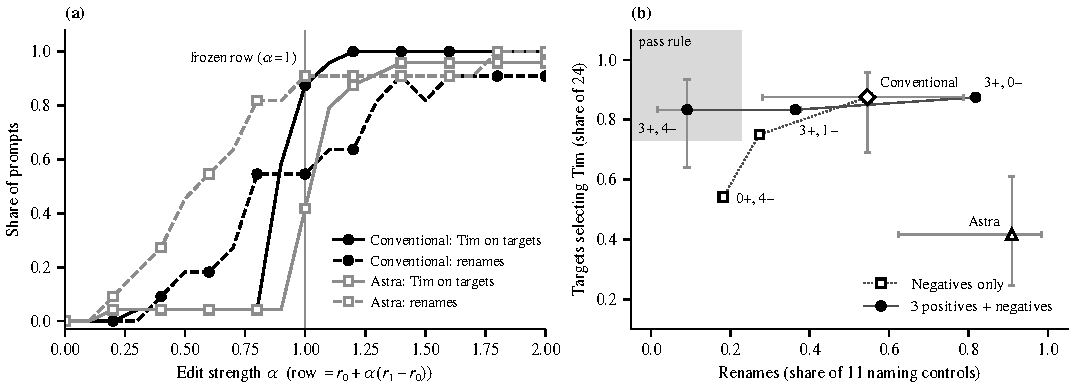
\includegraphics[width=\linewidth]{figures/edits.pdf}
\vspace{-14pt}
\caption{\textbf{One-row edits generalize to a slot.} (a)~Scaling each frozen row toward the base. Solid lines: share of 24 unseen target prompts selecting \textit{Tim}. Dashed lines: share of 11 unseen naming controls whose output changed. (b)~Hits against naming leaks for the frozen rows and for contrastive fits with 0--8 negatives. Upper left is better.}
\label{fig:edits}
\end{figure}

\paragraph{The same holds on the diagnostic model.} Astra wrote a 380-byte edit to FLAN vocabulary row 852 so that a saved answer would begin with ``Now.'' It did, and the edit survived a witnessed power cycle. It also repeated ``Now'' later in the answer. A 512-byte row edit toward a correct ``queue-free'' answer fixed its development case but failed paraphrases and recovered-pool controls, so it was never promoted. Restore original reproduced every earlier answer byte for byte.

\subsection{Latency}
Figure~\ref{fig:latency}a fixes one saved incident (186 prompt tokens, 50 decoder steps, original weights) and changes only the execution path. Running only the output classifier on the FPGA took \latBaseline\,s. Moving every learned matrix (3{,}722 projections) onto the array cut this to \latArray\,s. C++ packing with a weight cache, resident vocabulary weights in 16\,MiB of FPGA-readable memory and a command queue brought it to about 49\,s. Every answer matched byte for byte. In the encoder and decoder projections the array was busy for only 26.7\% and 3.7\% of cycles, while DDR delivered a read beat in 27--30\%. The engine reads \weightGB\,GB of weights per answer. At one 64-bit read per 50\,MHz clock that alone takes \floorDdr\,s, against a \floorMac\,s arithmetic floor. Memory, not arithmetic, sets the limit.

Figure~\ref{fig:latency}b tracks three recordings and one new wording across decoder changes. Verifying groups of prompt-derived token proposals with the unchanged model~\cite{leviathan2023speculative,saxena2023prompt} cut the original checkpoint from \latScalarMin--\latScalarMax\,s to \latVerifyMin--\latVerifyMax\,s with identical text. On Queue history v2, batched fusion, NEON integer packing and native batched quantization brought complete answers to \latBestMin--\latBestMax\,s, with first text at 8.4--10.4\,s. In software, verifier passes fell from 138 to 82 across 18 frozen questions with every token unchanged. The board kept processing 147--186 live telemetry windows during each answer. Every cell is a single observation.

\begin{figure}[t]
\centering
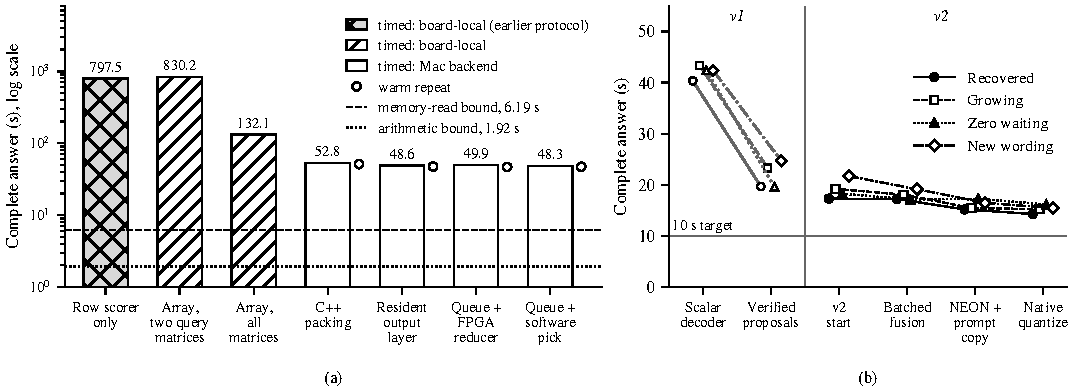
\includegraphics[width=\linewidth]{figures/latency.pdf}
\vspace{-14pt}
\caption{\textbf{Complete-answer latency on the physical PYNQ-Z2.} (a)~One saved incident with fixed weights and question. Only the execution path changes, and all answers are byte-identical. Pink lines are lower bounds at 50\,MHz. (b)~Three 60-reading recordings and one unfamiliar wording. The gray segment uses the original checkpoint. The black segment uses Queue history v2, so the two segments are not directly comparable. Single runs, timed from the Mac backend with polling.}
\label{fig:latency}
\end{figure}

\subsection{Diagnosis quality}
The first diagnostic FLAN candidate met all five answer requirements on 0 of 12 synthetic incidents. Its replacement passed 12 of 12 by direct review on fresh incidents and wordings. A frozen lexical scorer gave it 9 of 12, because it missed three uses of ``warns.'' On the board, the original checkpoint called a queue-free trace ``cleared.'' Numerical parity faithfully reproduced that error. Queue history v2 classified 15 of 15 independent frozen histories and 9 of 9 active-queue trends in the software reference. On the board it corrected the false recovery on the queue-free upload. Five of 12 archived recovery answers omitted an explicit current count of zero. Separately, the fixed-point telemetry forecaster changed 18 of 14{,}291 decisions compared with floating point, warning on 450 versus 451 of 772 queue episodes. Our rerun reproduced these figures exactly.

\begin{methods}[Limitations]
All telemetry is synthetic, so production accuracy is unmeasured. Latency cells are single runs on one board, with no variance estimate. The edit studies use one checkpoint and one target. In this 512-token vocabulary, \textit{Tim} and \textit{Lily} are the only names that encode as one token in context, so a second target name cannot be tested here. Astra produced one proposal, so we cannot separate its quality from sampling noise. We measured no power or energy, and we have no CPU-only or GPU baseline for the FLAN workload. Reproduction by a second developer and a power-cycle test of Queue history v2 remain open.
\end{methods}

\section{Conclusion}
A small Zynq-7020 FPGA board can serve a quantized language model with every learned matrix on the fabric and every score bit-exact. Its behavior can be changed and restored with a hash-guarded write of a few hundred bytes. The edits are real but blunt. A one-row edit attaches to the slot the token fills, not the concept around it, and small contrastive constraint sets largely fix that. Latency is bound by memory traffic: \weightGB\,GB of weight reads per answer. Next we will report:
\begin{enumerate}
\item \textbf{Memory path:} DMA burst scheduling and weight reuse to approach the \floorDdr\,s read floor, then a clock and lane study.
\item \textbf{Edit specificity at scale:} contrastive fits across more targets, more checkpoints and repeated Astra proposals with confidence intervals.
\item \textbf{Real telemetry:} a shadow deployment with per-case correctness, power and repeated latency.
\end{enumerate}

\vspace{2pt}
{\small\textbf{Reproduce.} \texttt{python3 paper/analysis.py} rebuilds every figure and number. \texttt{python3 -m paper.experiments.lm001\_extended} and \texttt{python3 -m paper.experiments.contrastive\_fit} rerun the new experiments in about 40\,s on a laptop. Each needs the pinned \texttt{run.c}, \texttt{tok512.bin} and \texttt{stories260K.ppq}. Board evidence is in \texttt{kit/evidence/} and \texttt{build/}.}

{\small
\begin{thebibliography}{9}\setlength{\itemsep}{0pt}
\bibitem{openai2026} OpenAI. Research acceleration: the jagged frontier. Technical report, November 2026.
\bibitem{karpathy2023llama2c} A.~Karpathy. llama2.c, commit 350e04f, 2023. \url{https://github.com/karpathy/llama2.c}
\bibitem{eldan2023tinystories} R.~Eldan and Y.~Li. TinyStories: How small can language models be and still speak coherent English? arXiv:2305.07759, 2023.
\bibitem{chung2022flan} H.~W.~Chung et al. Scaling instruction-finetuned language models. arXiv:2210.11416, 2022.
\bibitem{leviathan2023speculative} Y.~Leviathan, M.~Kalman and Y.~Matias. Fast inference from transformers via speculative decoding. ICML, 2023.
\bibitem{saxena2023prompt} A.~Saxena. Prompt lookup decoding, 2023. \url{https://github.com/apoorvumang/prompt-lookup-decoding}
\bibitem{wilson1927} E.~B.~Wilson. Probable inference, the law of succession, and statistical inference. JASA 22:209--212, 1927.
\end{thebibliography}}

\end{document}
